\documentclass[a4paper,12pt]{article}

\usepackage[latin1,utf8]{inputenc}       % Tipos de caracteres
\usepackage[portuges]{babel}             % Português
\usepackage[a4paper,portrait]{geometry}  % Tipo de papel
\usepackage{graphicx}                    % Gráficos

\topmargin = 10pt                        % Margem superior: 20pt  
\textheight = 622pt                      % Altura do texto: 592pt

\begin{document}

%\epsfysize=5.0truecm\epsffile{imagens/Figura01.eps}
%
% Inclusão de Imagens
%
%    \includegraphics[attr1=val1, attr2=val2, ..., attrn=valn]{imagename}
%
% Exemplos:
%    \includegraphics[width=\textwidth]{imagefile.pdf}
%    \includegraphics[width=5cm,height=5cm,keepaspectratio]{imagefile.pdf}
%    \includegraphics[width=5cm,height=5cm]{imagefile.pdf}
%

\begin{figure}[h]
\begin{center}
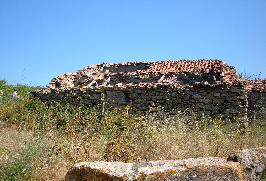
\includegraphics[width=6cm,height=6cm,keepaspectratio]{dscf1683b_v1.jpg}
\end{center}
\caption{Figura com legenda}
\end{figure}

\begin{figure}[h]
\begin{center}
\reflectbox{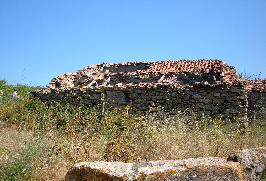
\includegraphics[width=6cm,height=7cm,keepaspectratio]{dscf1683b_v1.jpg}}
\end{center}
\caption{Figura refletida}
\end{figure}


\end{document}
